% ===========================================================================
% MODELO DE RELATORIO  ·  ENE0046 Laboratorio de Eletronica  ·  2026/2
%
% Como usar
%   1. Preencha o bloco IDENTIFICACAO logo abaixo.
%   2. Deixe comentados os autores que nao existirem. Um autor fica centralizado,
%      dois dividem a linha, tres ocupam tercos.
%   3. Substitua o texto de cada secao pelo seu. As orientacoes que estao la
%      dizem o que se espera em cada uma.
%   4. Compile com pdflatex duas vezes, ou com latexmk -pdf.
%
% Estrutura
%   Roteiro 1 nao tem bancada: use so a subsecao 4.1 e a 5.1, e compare o calculo
%   analitico com a simulacao de projeto.
%   Roteiros 2 a 7 usam a estrutura inteira.
%
% O arquivo estilo-relatorio.tex e a imagem logo-unb.png devem estar na mesma
% pasta deste arquivo.
% ===========================================================================
\documentclass[11pt,a4paper]{article}
% !TeX root = modelo-relatorio.tex
% Formatacao do relatorio. Compile o modelo-relatorio.tex, nao este arquivo.
\usepackage[T1]{fontenc}
\usepackage[utf8]{inputenc}
\usepackage[brazil]{babel}
\usepackage[a4paper,top=1.6cm,bottom=1.8cm,left=2.1cm,right=2.1cm]{geometry}
\usepackage[default]{lato}
\usepackage{amsmath,amssymb}
\usepackage{siunitx}
\usepackage{graphicx}
\usepackage{booktabs,array,longtable,colortbl}
\usepackage{enumitem}
\usepackage{tcolorbox}
\usepackage{xcolor}
\usepackage{tikz}
\usepackage{titlesec}
\usepackage{fancyhdr}
\usepackage{caption}
\usepackage{etoolbox}
\usepackage[colorlinks=true,linkcolor=azul,urlcolor=azul,citecolor=azul]{hyperref}
\tcbuselibrary{skins,breakable}

\definecolor{azul}{HTML}{0A4B8C}
\definecolor{azulclaro}{HTML}{E8F0F8}
\definecolor{verde}{HTML}{0B7A4B}
\definecolor{cinza}{HTML}{5B6672}
\definecolor{cinzaclaro}{HTML}{F4F6F8}
\definecolor{vinho}{HTML}{B04A4A}
\definecolor{vinhoclaro}{HTML}{FBF2F2}

\sisetup{output-decimal-marker={,}, per-mode=symbol}
\setlength{\parindent}{0pt}
\setlength{\parskip}{6pt plus 1pt}
\setlist{itemsep=3pt, topsep=4pt, parsep=0pt, leftmargin=1.3em}
\renewcommand{\arraystretch}{1.25}
\linespread{1.06}

% ---- secoes numeradas com marcador colorido -------------------------------
\titleformat{\section}[hang]
  {\Large\bfseries\color{azul}}
  {\raisebox{-1pt}{\tikz\node[fill=azul,text=white,rounded corners=2pt,
     inner sep=3pt,minimum width=20pt,align=center]{\bfseries\thesection};}}
  {10pt}{}
\titlespacing*{\section}{0pt}{16pt plus 3pt}{6pt}
\titleformat{\subsection}{\large\bfseries\color{cinza}}{\thesubsection}{8pt}{}
\titlespacing*{\subsection}{0pt}{11pt plus 2pt}{3pt}

% ---- legendas -------------------------------------------------------------
\captionsetup{font=small,labelfont={bf,color=azul},labelsep=period,skip=6pt}

% ---- identificacao --------------------------------------------------------
\newcommand{\autorA}{}\newcommand{\matA}{}
\newcommand{\autorB}{}\newcommand{\matB}{}
\newcommand{\autorC}{}\newcommand{\matC}{}
\newcommand{\autorum}[2]{\renewcommand{\autorA}{#1}\renewcommand{\matA}{#2}}
\newcommand{\autordois}[2]{\renewcommand{\autorB}{#1}\renewcommand{\matB}{#2}}
\newcommand{\autortres}[2]{\renewcommand{\autorC}{#1}\renewcommand{\matC}{#2}}

\newcommand{\disciplina}{ENE0046 · Laboratório de Eletrônica}
\newcommand{\semestre}{2026/2}
\newcommand{\turma}{}
\newcommand{\roteironum}{}
\newcommand{\roteirotema}{}
\newcommand{\aturma}[1]{\renewcommand{\turma}{#1}}
\newcommand{\roteiro}[2]{\renewcommand{\roteironum}{#1}\renewcommand{\roteirotema}{#2}}

\newcommand{\umautor}[2]{%
  \begin{minipage}[t]{\dimexpr\linewidth-4pt\relax}\centering
    \parbox[t][30pt][t]{\linewidth}{\centering
      {\fontsize{10.5}{12.5}\selectfont #1}}\\[-2pt]
    {\color{cinza}\fontsize{9}{11}\selectfont\texttt{#2}}
  \end{minipage}}

\newcounter{nautores}
\newcommand{\blocoautores}{%
  \setcounter{nautores}{0}%
  \ifdefempty{\autorA}{}{\stepcounter{nautores}}%
  \ifdefempty{\autorB}{}{\stepcounter{nautores}}%
  \ifdefempty{\autorC}{}{\stepcounter{nautores}}%
  \ifnum\value{nautores}=0
    \begin{center}\color{vinho}\bfseries
      Preencha ao menos um autor no preâmbulo do arquivo.
    \end{center}
  \else
    \begin{center}
    \ifcase\value{nautores}\or
      % --- um autor: ocupa o centro
      \begin{minipage}{0.5\textwidth}\umautor{\autorA}{\matA}\end{minipage}%
    \or
      % --- dois autores: metades
      \begin{minipage}{0.42\textwidth}\umautor{\autorA}{\matA}\end{minipage}\hspace{0.04\textwidth}%
      \begin{minipage}{0.42\textwidth}\umautor{\autorB}{\matB}\end{minipage}%
    \or
      % --- tres autores: tercos
      \begin{minipage}{0.31\textwidth}\umautor{\autorA}{\matA}\end{minipage}\hspace{0.015\textwidth}%
      \begin{minipage}{0.31\textwidth}\umautor{\autorB}{\matB}\end{minipage}\hspace{0.015\textwidth}%
      \begin{minipage}{0.31\textwidth}\umautor{\autorC}{\matC}\end{minipage}%
    \fi
    \end{center}
  \fi}

% ---- cabecalho do relatorio -----------------------------------------------
\newcommand{\capa}{%
\begin{tcolorbox}[colback=azul,colframe=azul,boxrule=0pt,arc=4pt,
  left=16pt,right=16pt,top=13pt,bottom=13pt]
\color{white}
\begin{minipage}{0.76\textwidth}
  {\fontsize{9}{11}\selectfont\textbf{\MakeUppercase{\disciplina{} · \semestre{}}}}\\[6pt]
  {\fontsize{22}{25}\selectfont\bfseries Relatório do Roteiro \roteironum}\\[3pt]
  {\fontsize{12.5}{15}\selectfont \roteirotema}
\end{minipage}\hfill
\begin{minipage}{0.2\textwidth}\raggedleft
  \colorbox{white}{\hspace{2pt}\raisebox{-2pt}{
\includegraphics[height=30pt]{logo-unb.png}}\hspace{2pt}}
\end{minipage}
\end{tcolorbox}
\vspace{10pt}
\blocoautores
\ifdefempty{\turma}{}{%
  \begin{center}{\color{cinza}\fontsize{9}{11}\selectfont Turma \turma}\end{center}}
\vspace{4pt}
{\color{azulclaro}\hrule height 2pt}
\vspace{2pt}}

% ---- caixas auxiliares ----------------------------------------------------
\newtcolorbox{formula}{colback=azulclaro,colframe=azul,boxrule=0.8pt,arc=3pt,
  left=12pt,right=12pt,top=9pt,bottom=9pt}
\newtcolorbox{nota}[1]{colback=cinzaclaro,colframe=cinza,boxrule=0.8pt,arc=3pt,
  left=10pt,right=10pt,top=7pt,bottom=7pt,
  title={\textbf{#1}},fonttitle=\small\bfseries,coltitle=white,colbacktitle=cinza}
\newenvironment{resumo}
  {\vspace{6pt}\begin{center}\begin{minipage}{0.92\textwidth}
   \begin{tcolorbox}[colback=cinzaclaro,colframe=cinzaclaro,boxrule=0pt,arc=3pt,
     left=14pt,right=14pt,top=10pt,bottom=10pt,
     borderline west={2.5pt}{0pt}{azul}]
   {\color{azul}\fontsize{8}{10}\selectfont\textbf{RESUMO}}\\[4pt]
   \small}
  {\end{tcolorbox}\end{minipage}\end{center}\vspace{2pt}}

\newtcolorbox{espec}{colback=azulclaro,colframe=azul,boxrule=0.8pt,arc=3pt,
  left=12pt,right=12pt,top=9pt,bottom=9pt,
  title={\textbf{Especificação da matrícula}},fonttitle=\bfseries,
  coltitle=white,colbacktitle=azul}

% ---- rodape ---------------------------------------------------------------
\pagestyle{fancy}\fancyhf{}
\renewcommand{\headrulewidth}{0pt}
\renewcommand{\footrulewidth}{0.4pt}
\fancyfoot[L]{\color{cinza}\fontsize{8}{10}\selectfont \disciplina{} · \semestre{} · Roteiro \roteironum}
\fancyfoot[R]{\color{cinza}\fontsize{8}{10}\selectfont \thepage}

\newlist{referencias}{itemize}{1}
\setlist[referencias]{label={}, leftmargin=1.1em, itemindent=-1.1em,
                     itemsep=3pt, topsep=2pt, parsep=0pt}

\newcommand{\mat}[1]{\texttt{\textbf{#1}}}


% --------------------------- IDENTIFICACAO ---------------------------------
\roteiro{3}{Amplificador Operacional: Não-idealidades}
\aturma{01}

\autorum{Bernardo Manciola Lobo}{21/1026486}
\autordois{Enzo Morrone de Azevedo Muniz}{22/1035442}
\autortres{Matheus Vieira Tiveron}{24/1039879}
% ---------------------------------------------------------------------------

\begin{document}
\capa

\begin{resumo}
Escreva este parágrafo por último, com 100 a 150 palavras. Diga o que você projetou, sob
qual especificação, o que simulou ou mediu, o principal resultado numérico e a que
conclusão chegou. Quem ler só este parágrafo deve saber o que você fez e o que encontrou.
\end{resumo}

\section{Introdução}

Amplificadores operacionais são componentes muito úteis, por isso, são tema de diversas disciplinas dos cursos de engenharia.
Por isso, por motivos de simplificação, muitas vezes são apresentados como componentes "perfeitos" tendo caracteristicas como:
ganho infinito, resistensia de entrada infinita, curto virtual entre as entradas, entre outros.
Essas caracteristicas são apenas aproximações, que não condizem com o mundo real. Assim, existem "imperfeições", não idealidades. Algumas delas, são problemas para as suas aplicações, já outras, aproveitam dessas imperfeições.

Um exemplo onde a não idealidade atrapalha é a tensão de offset em aparelhos de eletrocardiograma.
Em um eletrocardiograma simplificadamente, o objetivo é comparar o potencial em dois eletrodos (esquerdo e direito) posicionados no corpo humano e desta forma inferir os sinais eletricos que são gerados com o batimento do coração.
O problema é que os sinais eletricos gerados são extremamente pequenos, e a tensão de offset do amplificador, a qual só é aplicada em um dos eletrodos e mesmo podendo ser poucos mili volts, quando amplificada, faz dois sinais iguais ter uma grande diferença - atrapalhando a interpretação dos sinais. Esse problema é resolvível caso a tensão de offset seja conhecida.

Um outro exemplo onde a não idealidade agora pode ser benéfica, é o efeito do slew rate na distorção de sinais de ondas sonoras.
Guitarristas, principalmente, apreciam a distorção do sinal sonoro para a criação de novas notas musicais. 
Comparado com diodos, os quais funcionam "cortando" os sinais mais potentes, por exemplo, amplificadores operacionais permitem atingir uma distorção mais suave ao transformar as ondas senoidais do sinal sonoro em ondas triangulares por meio do slew rate. Para essa amplicação, amplificadores com slew rate baixo, uma característica ruim na maioria dos contextos, são preferidos aos outros com slew rate muito grande.

Assim, foram escolhidos 4 não idealidades para investigar: a tensão de offset, a corrente de polarização, a resposta em frequência e o slew rate. Esses parametros serão estudados nos circuitos integrados LM741 e TL064, ambos da Texas Intruments.
O objetivo deste relatório é discutir, medir e verificar essas 4 não idealidades. 
O texto está organizado nas secções: Fundamentação teórica, Especificação e projeto, Metodologia, Simulação e Resultados.

\section{Fundamentação Teórica}

Esta seção deduz as expressões usadas no projeto e na análise dos quatro ensaios. As hipóteses de amplificador ideal — ganho infinito, impedâncias de entrada infinitas, impedância de saída nula, offset nulo e banda infinita — são abandonadas uma a uma, e cada abandono gera uma expressão que será confrontada com a medição.

\subsection{Tensão de offset}

A assimetria do par de entrada equivale a uma fonte contínua $V_{os}$ em série com uma das entradas. No amplificador não inversor de ganho $G$, com a entrada não inversora aterrada, essa fonte é amplificada como se fosse sinal, e a saída fica

\begin{equation}
V_o = G \, V_{os} \qquad \Rightarrow \qquad V_{os} = \frac{V_o}{G} .
\label{eq:offset}
\end{equation}

No ensaio da Seção~2.1, $G = 101$, com $R_f = \SI{100}{\kilo\ohm}$ e $R_g = \SI{1}{\kilo\ohm}$, de modo que a tensão de offset do modelo é a saída dividida por 101.

\subsection{Corrente de polarização}

As entradas drenam uma corrente contínua $I_b$. Sobre a resistência vista pela entrada, essa corrente produz uma tensão que se soma ao offset. Com um resistor $R_s$ entre o terra e a entrada não inversora, a tensão nessa entrada passa a $-I_b R_s$ (o sinal depende do sentido da corrente), e a saída fica

\begin{equation}
V_o = G \left( V_{os} - I_b R_s \right) .
\label{eq:polarizacao}
\end{equation}

A diferença entre a saída com $R_s$ e a saída sem $R_s$ isola o termo da corrente:

\begin{equation}
\Delta V_o = -G \, I_b \, R_s \qquad \Rightarrow \qquad I_b = \frac{\Delta V_o}{G \, R_s} .
\label{eq:ib}
\end{equation}

Com $G = 101$ e $R_s = \SI{100}{\kilo\ohm}$, a corrente de polarização é a variação da saída dividida por $101 \times 100$ kΩ.

\subsection{Resposta em frequência}

O ganho em malha aberta cai com a frequência como um passa-baixas de primeira ordem, com um produto ganho por banda constante, o \textit{GBW}. Com a realimentação fixando o ganho em $G$, a frequência de corte do estágio é

\begin{equation}
f_c = \frac{\text{GBW}}{G} .
\label{eq:fc}
\end{equation}

A resposta em frequência do estágio realimentado é

\begin{equation}
A(f) = \frac{G}{\sqrt{1 + (f/f_c)^2}} ,
\label{eq:resposta}
\end{equation}

de modo que, em $f = f_c$, o ganho cai a $1/\sqrt{2} \approx 0{,}707$ do valor em baixa frequência. Multiplicando $G$ por $f_c$ recupera-se o produto ganho por banda, que deve ser o mesmo para os dois ganhos do mesmo amplificador.

\subsection{Slew rate}

A saída não varia mais rápido que o slew rate $SR$. Uma senoide de amplitude $V_p$ e frequência $f$ exige, na passagem por zero, uma taxa de variação

\begin{equation}
\left. \frac{dv_o}{dt} \right|_{\max} = 2\pi f V_p .
\label{eq:slew}
\end{equation}

Quando essa taxa ultrapassa o slew rate do amplificador, a saída deixa de ser senoide e vira triângulo. A frequência a partir da qual isso ocorre é

\begin{equation}
f_{\max} = \frac{SR}{2\pi V_p} .
\label{eq:fmax}
\end{equation}

Diferentemente da largura de banda, que é linear, o limite por slew rate depende da amplitude: quanto maior $V_p$, menor a frequência em que a distorção aparece.

\section{Especificação e Projeto}

Esta seção transcreve a especificação numérica de cada integrante, calculada a partir dos nove dígitos da matrícula, e leva cada parâmetro até o valor de componente na série E12.

\subsection{Especificação da equipe}

A equipe~2 adotou, para a bancada, o ganho baixo $G_1 = 13$ e a amplitude de pico $V_p = \SI{2,5}{\volt}$. O ganho alto é $G_2 = 101$ para todas as equipes, com $R_f = \SI{100}{\kilo\ohm}$ e $R_g = \SI{1}{\kilo\ohm}$.

\begin{table}[h]
\centering
\caption{Especificação da equipe~2.}
\label{tab:equipe_r3}
\begin{tabular}{lc}
\hline
Grandeza & Valor \\
\hline
$G_1$ (ganho baixo) & 13 \\
$G_2$ (ganho alto) & 101 \\
$V_p$ (slew rate) & \SI{2,5}{\volt} \\
$R_f$ (ganho 101) & \SI{100}{\kilo\ohm} \\
$R_g$ (ganho 101) & \SI{1}{\kilo\ohm} \\
\hline
\end{tabular}
\end{table}

\subsection{Especificação individual}

Cada integrante recebeu uma especificação distinta, derivada da própria matrícula. A Tabela~\ref{tab:individuais_r3} reúne os parâmetros calculados.

\begin{table}[h]
\centering
\caption{Especificação individual dos integrantes.}
\label{tab:individuais_r3}
\begin{tabular}{lccc}
\hline
Grandeza & 211026486 & 221035442 & 241039879 \\
\hline
$EF$ & 26 & 35 & 39 \\
$GH$ & 48 & 44 & 87 \\
$I$ & 6 & 2 & 9 \\
$G_1$ & 25 & 20 + 14 = 34 & 20 + 18 = 38 \\
$G_2$ & 87 & 83 & 80 + 5 = 85 \\
$V_p$ & 5,0 & 3,0 & 6,5 \\
\hline
\end{tabular}
\end{table}

\subsection{Projeto dos resistores}

\subsubsection{Ganho alto ($G_2 = 101$)}

Fixo para todas as equipes: $R_f = \SI{100}{\kilo\ohm}$ e $R_g = \SI{1}{\kilo\ohm}$, o que dá $G_2 = 1 + 100/1 = 101$.

\subsubsection{Ganho baixo ($G_1$ da equipe = 13)}

Com um resistor por perna, entre os valores do laboratório, procura-se o par que realize $G_1 = 13$. A combinação escolhida é $R_f = \SI{12}{\kilo\ohm}$ e $R_g = \SI{1}{\kilo\ohm}$.


\subsubsection{Ganhos individuais}

Na etapa de simulação, cada integrante projeta seu próprio par de resistores para $G_1$ e $G_2$, conforme a Tabela~\ref{tab:individuais_r3}.

\begin{table}[htbp]
    \centering
    \caption{Dimensionamento dos resistores e ganhos para cada integrante.}
    \label{tab:resistores_integrantes}
    \resizebox{\textwidth}{!}{%
    \begin{tabular}{cccccccc}
        \toprule
        \textbf{Integrante (Matrícula)} & \textbf{Parâmetro} & \textbf{Ganho Teórico (\(G\))} & \textbf{\(R_f\) Adotado} & \textbf{\(R_g\) Adotado} & \textbf{Ganho Real} & \textbf{Desvio (\%)} \\
        \midrule
        \multirow{2}{*}{211026486} 
             & \(G_1\) (Baixo) & 25 & \(12\,\text{k}\Omega + 12\,\text{k}\Omega\) & \(1\,\text{k}\Omega\) & 25,00 & 0,00\% \\
             & \(G_2\) (Alto)  & 87 & \(18\,\text{k}\Omega + 68\,\text{k}\Omega\) & \(1\,\text{k}\Omega\) & 87,00 & 0,00\% \\
        \midrule
        \multirow{2}{*}{221035442} 
             & \(G_1\) (Baixo) & 34 & \(33\,\text{k}\Omega\) & \(1\,\text{k}\Omega\) & 34,00 & 0,00\% \\
             & \(G_2\) (Alto)  & 83 & \(82\,\text{k}\Omega\) & \(1\,\text{k}\Omega\) & 83,00 & 0,00\% \\
        \midrule
        \multirow{2}{*}{241039879} 
             & \(G_1\) (Baixo) & 38 & \(10\,\text{k}\Omega + 27\,\text{k}\Omega\) & \(1\,\text{k}\Omega\) & 38,00 & 0,00\% \\
             & \(G_2\) (Alto)  & 85 & \(2{,}7\,\text{k}\Omega + 82\,\text{k}\Omega\) & \(1\,\text{k}\Omega\) & 85,70 & 0,82\% \\
        \bottomrule
    \end{tabular}%
    }
\end{table}

\section{Metodologia}

Conte o que você fez e com quais parâmetros, de modo que um colega consiga repetir sem
precisar perguntar nada. Explique as escolhas que não são evidentes: por que essa faixa de
varredura, por que esse passo de integração, por que esse intervalo de gravação.

Inclua a figura do esquemático, com legenda que descreva o que ela mostra, e cite-a no
texto, como na Figura~\ref{fig:exemplo}. Se uma figura não for mencionada em nenhum
parágrafo, ela provavelmente não precisa estar aqui.

\subsection{Simulação de projeto, uma por integrante}

\subsubsection{Tensão de offset (241039879)}

O arquivo \texttt{item\_1.asc} contém o amplificador não inversor de ganho 101, com $R_f = \SI{100}{\kilo\ohm}$ e $R_g = \SI{1}{\kilo\ohm}$, e a entrada não inversora ligada ao terra. Esse ganho é fixo para todos os integrantes, porque o mesmo circuito é usado no ensaio de corrente de polarização da Seção~2.2 e a montagem é uma só. A análise é de ponto de operação (\texttt{.op}), conforme o roteiro. O esquemático está na Figura~\ref{fig:item1_esquema}.

Com as duas entradas no mesmo potencial (ambas em zero), a saída de um amplificador real não é zero, porque a assimetria do par de entrada equivale a uma fonte contínua $V_{os}$ em série com uma das entradas. Essa fonte é amplificada pelo ganho do estágio, de modo que a tensão de offset do modelo é

\begin{equation}
V_{os} = \frac{|V_o|}{101} .
\label{eq:offset_membro2}
\end{equation}

A saída simulada foi $V_o = \SI{-95,26}{\milli\volt}$, o que dá uma tensão de offset de $V_{os} = \SI{0,943}{\milli\volt}$. Esse valor está ligeiramente abaixo da faixa típica do datasheet do LM741, que é de \SI{1}{\milli\volt} a \SI{5}{\milli\volt}. A diferença de \SI{0,057}{\milli\volt} em relação ao limite inferior não indica erro de projeto: o datasheet dá valores típicos e máximos, e o modelo do LTspice foi ajustado para um valor de offset próximo de \SI{1}{\milli\volt} com sinal negativo. O módulo é o que interessa para a análise, e ele está dentro da ordem de grandeza esperada para o LM741. O sinal negativo indica apenas que a fonte de offset está com a polaridade invertida em relação à convenção adotada.

\begin{table}[h]
\centering
\caption{Simulação de offset do integrante 241039879.}
\label{tab:offset_membro2}
\begin{tabular}{lcc}
\hline
Grandeza & Valor simulado & Faixa do datasheet \\
\hline
$V_o$ & \SI{95,26}{\milli\volt} & --- \\
$V_{os} = |V_o|/101$ & \SI{0,943}{\milli\volt} & \SI{1}{\milli\volt} a \SI{5}{\milli\volt} \\
\hline
\end{tabular}
\end{table}

\subsubsection{Corrente de polarização}

\subsubsection{Resposta em frequência (211026486)}

O arquivo \texttt{item\_3.asc} contém dois amplificadores não inversores com o LM741, alimentados pela mesma fonte de sinal, com os ganhos $G_1 = 25$ e $G_2 = 87$ da matrícula 211026486. O primeiro estágio usa $R_1 = \SI{22}{\kilo\ohm}$ e $R_2 = \SI{2,2}{\kilo\ohm}$ em série na realimentação, com $R_3 = \SI{1}{\kilo\ohm}$ no ramo inferior, o que dá $G_1 = 1 + 24{,}2/1 = 25{,}2$. O segundo usa $R_4 = \SI{68}{\kilo\ohm}$ e $R_5 = \SI{18}{\kilo\ohm}$ em série na realimentação, com $R_6 = \SI{1}{\kilo\ohm}$ no ramo inferior, o que dá $G_2 = 1 + 86/1 = 87{,}0$. A diretiva de análise é \texttt{.ac dec 50 10 10Meg}, conforme o roteiro. O esquemático está na Figura~\ref{fig:item3_esquema}, e as curvas de ganho e fase estão na Figura~\ref{fig:item3_ac}.

No estágio de ganho baixo, o ganho em baixa frequência é de \SI{28}{\decibel}, que corresponde a $20 \log_{10}(25{,}2) = 28{,}03$~dB, e a curva começa a cair por volta de \SI{10}{\kilo\hertz}, com o cruzamento de $-3$~dB em relação ao valor de baixa frequência em torno de \SI{40}{\kilo\hertz}. No estágio de ganho alto, o ganho em baixa frequência é de \SI{39}{\decibel}, que corresponde a $20 \log_{10}(87) = 38{,}79$~dB, e o cruzamento de $-3$~dB ocorre em torno de \SI{12}{\kilo\hertz}. As fases acompanham: cada curva parte de $0^\circ$, passa por $-45^\circ$ na frequência de corte e tende a $-90^\circ$ uma década acima.

O produto ganho por banda dos dois estágios é aproximadamente o mesmo: $25{,}2 \times 40~\text{kHz} \approx \SI{1,0}{\mega\hertz}$ e $87 \times 12~\text{kHz} \approx \SI{1,0}{\mega\hertz}$. Esse valor coincide com o GBW típico do LM741 segundo o datasheet, o que confirma que a frequência de corte do estágio realimentado segue a equação~\eqref{eq:fc} e que o produto ganho por banda é constante para o mesmo amplificador. Os valores exatos das frequências de corte, lidos no cursor do LTspice, estão na Tabela~\ref{tab:fc_sim}.

\begin{figure}[h]
\centering
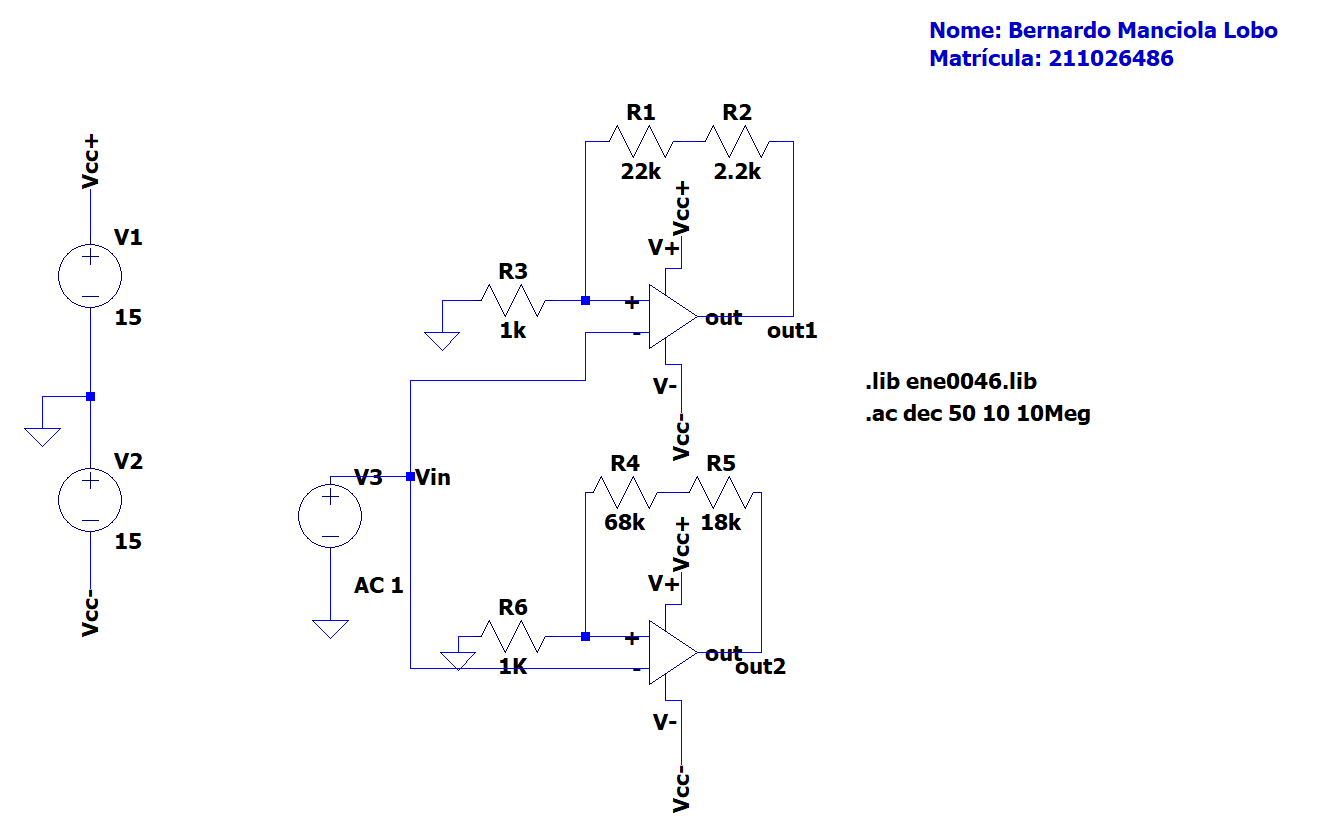
\includegraphics[width=0.9\textwidth]{montagem_sim_3.png}
\caption{Esquemático do \texttt{item\_3.asc}, com os dois amplificadores não inversores de ganhos $G_1 = 25{,}2$ e $G_2 = 87{,}0$.}
\label{fig:item3_esquema}
\end{figure}

\begin{figure}[h]
\centering
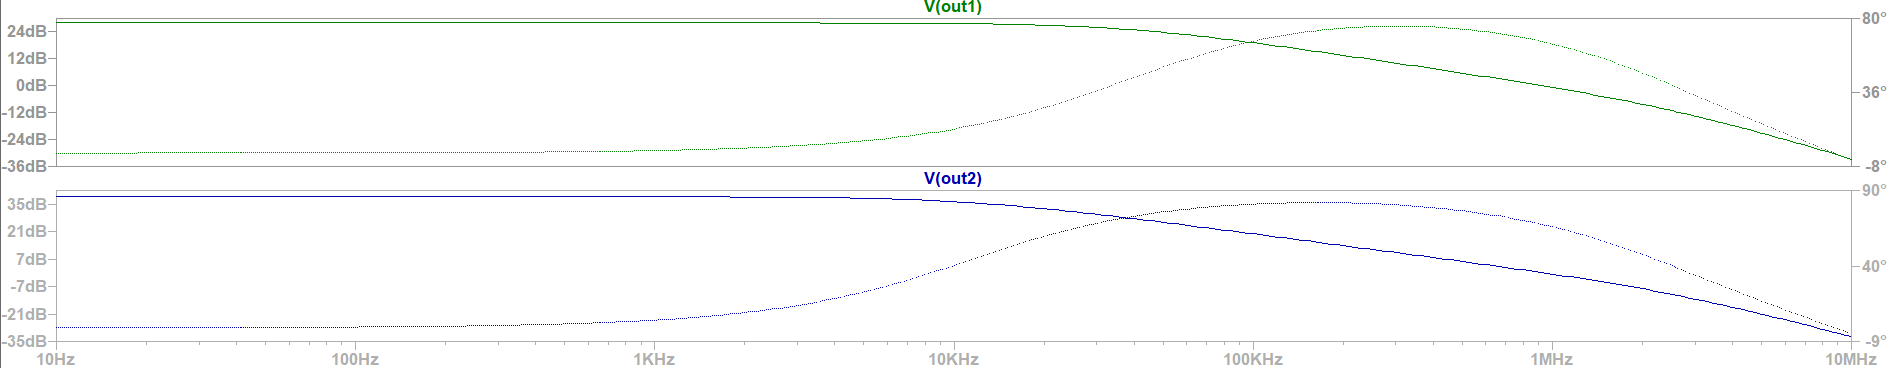
\includegraphics[width=0.9\textwidth]{resultado_sim_3.png}
\caption{Resposta em frequência do \texttt{item\_3.asc}: ganho (curvas superiores) e fase (curvas inferiores) dos dois estágios.}
\label{fig:item3_ac}
\end{figure}

\begin{table}[h]
\centering
\caption{Frequências de corte simuladas no \texttt{item\_3.asc}.}
\label{tab:fc_sim}
\begin{tabular}{lcccc}
\hline
Estágio & $G$ realizado & $f_c$ (simulado) & $G \cdot f_c$ & GBW datasheet \\
\hline
1 & 25,2 & \SI{40}{\kilo\hertz} & \SI{1,01}{\mega\hertz} & \SI{1}{\mega\hertz} \\
2 & 87,0 & \SI{12}{\kilo\hertz} & \SI{1,04}{\mega\hertz} & \SI{1}{\mega\hertz} \\
\hline
\end{tabular}
\end{table}

\subsection{Montagem em bancada - Elementos usados}

A equipe montou o circuito correspondente à especificação da equipe~2: ganho baixo $G_1 = 13$ e amplitude de pico $V_p = \SI{2,5}{\volt}$. O ganho alto é $G_2 = 101$ para todas as equipes, com $R_f = \SI{100}{\kilo\ohm}$ e $R_g = \SI{1}{\kilo\ohm}$, porque é também o ganho do ensaio de offset e a montagem é uma só. Antes de inserir cada resistor no protoboard, mediu-se o valor real com o multímetro; as tabelas abaixo registram esses valores, que são os usados nas contas do relatório. A alimentação seguiu a Seção~3.2 do roteiro: o par rastreado da fonte forneceu os \SI{\pm 15}{\volt}, com capacitores de desacoplamento de \SI{100}{\nano\farad} entre cada alimentação e o terra, junto aos pinos; as senoides vieram do gerador configurado para carga de alta impedância; e o comum do par rastreado, o terra do gerador e o da ponta do osciloscópio foram ligados ao mesmo ponto do protoboard. O multímetro, em tensão contínua, mediu as Seções~3.3 e~3.4, e o osciloscópio, com os dois canais, mediu as demais.

\subsubsection{Tensao de offset}

Montou-se o não inversor com $R_f = \SI{100}{\kilo\ohm}$ e $R_g = \SI{1}{\kilo\ohm}$, com a entrada não inversora ligada ao terra por um fio, e não deixada em aberto. Mediu-se a tensão contínua na saída com o multímetro e dividiu-se por 101 para obter a tensão de offset. Os valores dos componentes medidos estão na Tabela~\ref{tab:offset_comp}.

\begin{center}
\begin{tabular}{@{}lrrrr@{}}
\toprule
\label{tab:offset_comp}
\textbf{Grandeza} & \textbf{Nominal} & \textbf{Medido} & \textbf{Erro} \\
\midrule
  $R_f$ & $\SI{100}{\kilo\ohm}$ & $\SI{98,62}{\kilo\ohm}$ & -1,38\% \\
  $R_g$ & $\SI{1}{\kilo\ohm}$ & $\SI{1}{\kilo\ohm}$ & 0,00\% \\
  $C_{est}$ & $\SI{100}{\nano\farad}$ & $\SI{98}{\nano\farad}$ & -2,00\% \\
\bottomrule
\end{tabular}
\end{center}

\subsubsection{Corrente de polarização}

Substituiu-se o fio da entrada não inversora por um resistor de \SI{100}{\kilo\ohm} ao terra e mediu-se de novo a saída. A diferença entre as duas leituras, dividida por 101 e por \SI{100}{\kilo\ohm}, é a corrente de polarização. O mesmo procedimento foi repetido com o TL064. Os valores dos componentes medidos estão na Tabela~\ref{tab:ib_comp}.

\begin{center}
\begin{tabular}{@{}lrrrr@{}}
\toprule
\label{tab:ib_comp}
\textbf{Grandeza} & \textbf{Nominal} & \textbf{Medido} & \textbf{Erro} \\
\midrule
  $R_f$ & $\SI{100}{\kilo\ohm}$ & $\SI{98,62}{\kilo\ohm}$ & -1,38\% \\
  $R_g$ & $\SI{1}{\kilo\ohm}$ & $\SI{1}{\kilo\ohm}$ & 0,00\% \\
  $R_{parasita} $ & $\SI{100}{\kilo\ohm}$ & $\SI{100,7}{\kilo\ohm}$ & +0,70\% \\
  $C_{est}$ & $\SI{100}{\nano\farad}$ & $\SI{98}{\nano\farad}$ & -2,00\% \\
\bottomrule
\end{tabular}
\end{center}

\subsubsection{Resposta em frequência}

Montou-se o não inversor com o ganho baixo da equipe ($G_1 = 13$) e o não inversor com o ganho 101 ($G_2 = 101$). A senoide do gerador foi ajustada em \SI{100}{\hertz}, com amplitude tal que a saída tivesse \SI{200}{\milli\volt} de pico no ganho baixo e \SI{1}{\volt} de pico no ganho 101. Mantendo a entrada, subiu-se a frequência e mediu-se a amplitude da saída em seis a oito valores por curva. Os valores dos componentes medidos estão na Tabela~\ref{tab:fc_comp}.

\begin{center}
\begin{tabular}{@{}lrrrr@{}}
\toprule
\label{tab:fc_comp}
\textbf{Grandeza} & \textbf{Nominal} & \textbf{Medido} & \textbf{Erro} \\
\midrule
  $R_f$ & $\SI{12}{\kilo\ohm}$ & $\SI{11,74}{\kilo\ohm}$ & -2,17\% \\
  $R_g$ & $\SI{1}{\kilo\ohm}$ & $\SI{0,982}{\kilo\ohm}$ & -1,80\% \\

  $R_f$ & $\SI{10}{\kilo\ohm}$ & $\SI{10}{\kilo\ohm}$ & 0,00\% \\

  $R_{f2}$ & $\SI{100}{\kilo\ohm}$ & $\SI{98,60}{\kilo\ohm}$ & -1,40\% \\
  $R_{g2}$ & $\SI{1}{\kilo\ohm}$ & $\SI{0,985}{\kilo\ohm}$ & -1,50\% \\
\bottomrule
\end{tabular}
\end{center}

\subsubsection{Slew rate}

Montou-se o seguidor de tensão com o LM741 e aplicou-se uma senoide de \SI{1}{\kilo\hertz} com amplitude $V_p = \SI{2,5}{\volt}$ da equipe. Subiu-se a frequência até que a saída deixasse de ser senoide e virasse triângulo, e registrou-se essa frequência. Com os cursores do osciloscópio, mediu-se a inclinação da rampa em volt por microssegundo. O procedimento foi repetido com o TL064, subindo a frequência de novo até o triângulo aparecer. Não há componentes para medição nesta etapa.

\subsection{Simulação da montagem}

Refez-se a simulação com os valores de componente efetivamente usados na bancada, e não com os valores de projeto da Seção~4.1. O objetivo é separar duas causas de desvio que a medição sozinha não distingue: a tolerância dos componentes que a equipe pegou e o comportamento do circuito real que o modelo ideal não representa. Se a simulação da montagem se aproximar da medição, a diferença entre projeto e bancada vem quase toda da tolerância; se ela continuar distante, o que sobra aponta para algo fora do modelo, como a impedância da ponta de prova, a banda do amplificador ou a resistência de contato do protoboard. Os arquivos da Seção~4.1 foram reaproveitados, alterando apenas os valores dos resistores e, quando necessário, as amplitudes de entrada e eventuais erros na simulação inicial para coincidir com as ajustadas no gerador. Os valores medidos usados nesta seção estão nas Tabelas~\ref{tab:offset_comp}, \ref{tab:ib_comp} e \ref{tab:fc_comp}.

\subsubsection{Tensão de offset}

Na bancada, o não inversor de ganho 101 foi montado com $R_f = \SI{98,62}{\kilo\ohm}$ e $R_g = \SI{1,000}{\kilo\ohm}$, com a entrada não inversora aterrada. Repetiu-se a análise \texttt{.op} do \texttt{item\_1.asc} com esses valores, e a tensão de offset do modelo foi obtida dividindo a saída por $G = 1 + 98{,}62/1{,}000 = 99{,}62$

> **[INSERIR: com os valores medidos, o ganho não é mais 101. Recalcule $G = 1 + R_f/R_g$ com os valores medidos antes de dividir a saída para obter $V_{os}$. O valor de $V_{os}$ deve ser $V_o/G$, e não $V_o/101$.]**

Os resultados estão na Tabela~\ref{tab:offset_sim_bancada}.

\begin{table}[h]
\centering
\caption{Simulação da montagem: tensão de offset.}
\label{tab:offset_sim_bancada}
\begin{tabular}{lccc}
\hline
Peça & $V_o$ simulado & $V_{os}$ simulado & $V_{os}$ datasheet \\
\hline
LM741 & \SI{94,0}{\milli\volt} & \SI{0,9}{\milli\volt} & \SI{1}{\milli\volt} a \SI{5}{\milli\volt} \\
TL064 & \SI{2,7}{\milli\volt} & \SI{0,03}{\milli\volt} & \SI{3}{\milli\volt} a \SI{10}{\milli\volt} \\
\hline
\end{tabular}
\end{table}

\subsubsection{Corrente de polarização}

Na bancada, o resistor de entrada foi medido em \SI{100,7}{\kilo\ohm}, e os resistores de realimentação em \SI{98,62}{\kilo\ohm} e \SI{1,000}{\kilo\ohm}. Repetiu-se a análise \texttt{.op} do \texttt{item\_2.asc} (LM741) e do \texttt{item\_5.asc} (TL064) com esses valores, nas duas condições: com o resistor de entrada e com o fio. A corrente de polarização é obtida por

\begin{equation}
I_b = \frac{\Delta V_o}{G \, R_s} , \qquad G = 1 + \frac{R_f}{R_g} .
\label{eq:ib_sim_bancada}
\end{equation}

Os resultados estão na Tabela~\ref{tab:ib_sim_bancada}.

\begin{table}[h]
\centering
\caption{Simulação da montagem: corrente de polarização.}
\label{tab:ib_sim_bancada}
\begin{tabular}{lcccc}
\hline
Peça & $V_o$ sem $R_s$ & $V_o$ com $R_s$ & $\Delta V_o$ & $I_b$ \\
\hline
LM741 & \SI{0,09}{\volt} & \SI{1,12}{\volt} & \SI{1,03}{\volt} & \SI{10,4}{\milli\ampere} \\
TL064 & \SI{2,67}{\milli\volt} & \SI{2,67}{\milli\volt} & \SI{0,00}{\volt} & \SI{0,00}{\milli\ampere} \\
\hline
\end{tabular}
\end{table}

\subsubsection{Resposta em frequência}

Na bancada, os resistores do ganho baixo foram medidos em $R_f = \SI{11,74}{\kilo\ohm}$ e $R_g = \SI{0,982}{\kilo\ohm}$ (ou $R_f = \SI{10,000}{\kilo\ohm}$ e $R_g = \SI{0,982}{\kilo\ohm}$, conforme o par efetivamente montado), e os do ganho alto em $R_{f2} = \SI{98,60}{\kilo\ohm}$ e $R_{g2} = \SI{0,985}{\kilo\ohm}$. Repetiu-se a análise \texttt{.ac} do \texttt{item\_3.asc} com esses valores. Os ganhos realizados são $G_1 = 1 + 11{,}74/0{,}982 = 12{,}96$ e $G_2 = 1 + 98{,}60/0{,}985 = 101{,}10$. As frequências de corte e os produtos ganho por banda estão na Tabela~\ref{tab:fc_sim_bancada}.

\begin{table}[h]
\centering
\caption{Simulação da montagem: resposta em frequência.}
\label{tab:fc_sim_bancada}
\begin{tabular}{lcccc}
\hline
Estágio & $G$ realizado & $f_c$ simulado & $G \cdot f_c$ & GBW datasheet \\
\hline
Ganho baixo & 12,96 & \SI{74,49}{\kilo\hertz} & \SI{965,39}{\kilo\hertz} & \SI{1}{\mega\hertz} \\
Ganho alto & 101,10 & \SI{10,83}{\kilo\hertz} & \SI{1,09}{\mega\hertz} & \SI{1}{\mega\hertz} \\
\hline
\end{tabular}
\end{table}

\subsubsection{Slew rate}

Na bancada, o seguidor foi montado com $V_p = \SI{2,5}{\volt}$. Repetiu-se a análise \texttt{.tran} do \texttt{item\_4.asc} (LM741) e do \texttt{item\_6.asc} (TL064) com essa amplitude. Para o LM741, usaram-se as frequências de [INSERIR] e [INSERIR]; para o TL064, as de [INSERIR] e [INSERIR]. A inclinação da rampa foi medida no cursor do LTspice. Os resultados estão na Tabela~\ref{tab:sr_sim_bancada}.

\begin{table}[h]
\centering
\caption{Simulação da montagem: slew rate.}
\label{tab:sr_sim_bancada}
\begin{tabular}{lcccc}
\hline
Peça & $f$ da rampa & $SR$ simulado & $SR$ datasheet & $f_{\max}$ teórica \\
\hline
LM741 & \SI{30}{\kilo\hertz} & \SI{0,32}{\volt / \micro\second} & \SI{0,5}{\volt\per\micro\second} & \SI{31,8}{\kilo\hertz} \\
TL064 & \SI{200}{\kilo\hertz} & \SI{3,37}{\volt\per\micro\second} & \SI{3,5}{\volt\per\micro\second} & \SI{222,8}{\kilo\hertz} \\
\hline
\end{tabular}
\end{table}

\section{Resultados}

\subsection{Circuito montado}

Abaixo são apresentados os resultados numéricos obtidos no projeto analítico ideal, na simulação
da montagem e nas medições efetuadas na bancada. Os erros percentuais foram calculados tomando comoreferência a simulação da montagem.

\subsubsection{Tensao de offset - Resultados}

Para medir a tensão de offset, foi feito um amplificador não inversor com ganho de 101 e colocado a tensão das duas entradas sob o mesmo potencial.
Depois, a saída dividia por 101 é a tensão de offset.

\begin{center}
\begin{tabular}{@{}lrrrr@{}}
\toprule
\textbf{Grandeza} & \textbf{Projeto} & \textbf{Sim. montagem} & \textbf{Medido} &
\textbf{Erro} \\
\midrule
Tensao de offset LM741 & \SI{1}{\milli\volt} & \SI{1,09}{\milli\volt} & \SI{148,49}{\milli\volt} & \SI{372,29}{\percent} \\
Tensao de offset TL068 & \SI{3}{\milli\volt} & \SI{26}{\micro\volt} & \SI{2,663}{\milli\volt} & \SI{10342,3}{\percent} \\
\bottomrule
\end{tabular}
\end{center}

\subsubsection{Corrente de polarização - Resultados}

Para a corrente de polarização, pegou-se o experimento da tensão de offset e adicionou um resistor entre a entrada não inversora e a referencia,
para assim, com o valor da saída, calcular a corrente de polarização.

\begin{center}
\begin{tabular}{@{}lrrrr@{}}
\toprule
\textbf{Grandeza} & \textbf{Projeto} & \textbf{Sim. montagem} & \textbf{Medido} &
\textbf{Erro} \\
\midrule
Corrente de polarizacao LM741 & \SI{80}{\nano\ampere} & \SI{57,7}{\nano\ampere} & \SI{32,4}{\nano\ampere} & \SI{-56,14}{\percent} \\
Corrente de polarizacao TL068 & \SI{20}{\nano\ampere} & \SI{0}{\nano\ampere} & \SI{17,17}{\nano\ampere} & N/A \\
\bottomrule
\end{tabular}
\end{center}

\subsubsection{Resposta em frequencia - Resultados}

Para medir a resposta em frequencia, foi aplicado uma pequena tensão na entrada para as diferentes frequencias.

\begin{center}
\begin{tabular}{@{}lrrrr@{}}
\toprule
\textbf{Grandeza} & \textbf{Projeto} & \textbf{Sim. montagem} & \textbf{Medido} &
\textbf{Erro} \\
\midrule
  $G_1 = 0,707G_{1ideal}$ & & & & \\
  $G_2 = 0,707G_{2ideal}$ & & & & \\
\bottomrule
\end{tabular}
\end{center}

Com o ganho de 13, foi aplicado uma entrada de $V_{pp} = \SI{188}{\milli\volt} $

\begin{center}
\begin{tabular}{@{}lrrrr@{}}
\toprule
\textbf{Grandeza} & \textbf{Projeto} & \textbf{Sim. montagem} & \textbf{Medido} &
\textbf{Erro} \\
\midrule
$V_{out}$ de $G_1$ para \SI{100}{\hertz} & \SI{2444}{\milli\volt} & \SI{2444}{\milli\volt} & \SI{2440}{\milli\volt} & \SI{-0,16}{\percent} \\
$V_{out}$ de $G_1$ para \SI{14,51}{\kilo\hertz} & \SI{2444}{\milli\volt} & \SI{2401,7}{\milli\volt} & \SI{2320}{\milli\volt} & \SI{-3,40}{\percent} \\
$V_{out}$ de $G_1$ para \SI{28,92}{\kilo\hertz} & \SI{2444}{\milli\volt} & \SI{2287,7}{\milli\volt} & \SI{2040}{\milli\volt} & \SI{-10,83}{\percent} \\
$V_{out}$ de $G_1$ para \SI{43,33}{\kilo\hertz} & \SI{2444}{\milli\volt} & \SI{2129,4}{\milli\volt} & \SI{1760}{\milli\volt} & \SI{-17,35}{\percent} \\
$V_{out}$ de $G_1$ para \SI{57,74}{\kilo\hertz} & \SI{2444}{\milli\volt} & \SI{1954,6}{\milli\volt} & \SI{1560}{\milli\volt} & \SI{-20,19}{\percent} \\
$V_{out}$ de $G_1$ para \SI{72,5}{\kilo\hertz} & \SI{2444}{\milli\volt} & \SI{1778,5}{\milli\volt} & \SI{1320}{\milli\volt} & \SI{-25,78}{\percent} \\
$V_{out}$ de $G_1$ para \SI{115,3}{\kilo\hertz} & \SI{2444}{\milli\volt} & \SI{1356,3}{\milli\volt} & \SI{960}{\milli\volt} & \SI{-29,22}{\percent} \\
$V_{out}$ de $G_1$ para \SI{120}{\kilo\hertz} & \SI{2444}{\milli\volt} & \SI{1318,9}{\milli\volt} & \SI{960}{\milli\volt} & \SI{-27,21}{\percent} \\
\bottomrule
\end{tabular}
\end{center}

Com o ganho de 101, foi aplicado uma entrada de $V_{pp} = \SI{20}{\milli\volt} $

\begin{center}
\begin{tabular}{@{}lrrrr@{}}
\toprule
\textbf{Grandeza} & \textbf{Projeto} & \textbf{Sim. montagem} & \textbf{Medido} &
\textbf{Erro} \\
\midrule
$V_{out}$ de $G_2$ para \SI{100}{\hertz} & \SI{2020}{\milli\volt} & \SI{2020}{\milli\volt} & \SI{2120}{\milli\volt} & \SI{+4,95}{\percent} \\
$V_{out}$ de $G_2$ para \SI{14,51}{\kilo\hertz} & \SI{2020}{\milli\volt} & \SI{1138,5}{\milli\volt} & \SI{920}{\milli\volt} & \SI{-19,19}{\percent} \\
$V_{out}$ de $G_2$ para \SI{28,92}{\kilo\hertz} & \SI{2020}{\milli\volt} & \SI{654,2}{\milli\volt} & \SI{520}{\milli\volt} & \SI{-20,51}{\percent} \\
$V_{out}$ de $G_2$ para \SI{43,33}{\kilo\hertz} & \SI{2020}{\milli\volt} & \SI{449,9}{\milli\volt} & \SI{360}{\milli\volt} & \SI{-19,98}{\percent} \\
$V_{out}$ de $G_2$ para \SI{57,74}{\kilo\hertz} & \SI{2020}{\milli\volt} & \SI{341,3}{\milli\volt} & \SI{320}{\milli\volt} & \SI{-6,24}{\percent} \\
$V_{out}$ de $G_2$ para \SI{72,5}{\kilo\hertz} & \SI{2020}{\milli\volt} & \SI{273,3}{\milli\volt} & \SI{240}{\milli\volt} & \SI{-12,18}{\percent} \\
$V_{out}$ de $G_2$ para \SI{115,3}{\kilo\hertz} & \SI{2020}{\milli\volt} & \SI{172,8}{\milli\volt} & \SI{200}{\milli\volt} & \SI{+15,74}{\percent} \\
$V_{out}$ de $G_2$ para \SI{120}{\kilo\hertz} & \SI{2020}{\milli\volt} & \SI{166,1}{\milli\volt} & \SI{160}{\milli\volt} & \SI{-3,67}{\percent} \\
\bottomrule
\end{tabular}
\end{center}

\subsubsection{Slew Rate - Resultados}

Foi aplicado uma tensão senoide de $V_p = \SI{2,5}{\volt}$ na entrada, observado a frequencia onde a saída se tornava uma onda triangular e assim calculado o slew rate.

\begin{center}
\begin{tabular}{@{}lrrrr@{}}
\toprule
\textbf{Grandeza} & \textbf{Projeto} & \textbf{Sim. montagem} & \textbf{Medido} &
\textbf{Erro} \\
\midrule
Frequencia triangulo LM741 & \SI{45,2}{\kilo\hertz} & \SI{45,2}{\kilo\hertz} & \SI{42}{\kilo\hertz} & \SI{-7,08}{\percent} \\
Frequencia triangulo TL068 & \SI{180}{\kilo\hertz} & \SI{180}{\kilo\hertz} & \SI{150}{\kilo\hertz} & \SI{-16,67}{\percent} \\
Slew rate LM741 & \SI{0,5}{\volt/\micro\second} & \SI{0,50}{\volt/\micro\second} & \SI{0,48}{\volt/\micro\second} & \SI{-4,00}{\percent} \\
Slew rate TL068 & \SI{3,5}{\volt/\micro\second} & \SI{3,50}{\volt/\micro\second} & \SI{2,18}{\volt/\micro\second} & \SI{-37,71}{\percent} \\
\bottomrule
\end{tabular}
\end{center}

\section{Discussão}

\subsection{Projeto analítico e simulação de projeto}

O modelo ideal prevê offset e corrente de polarização nulos, banda infinita e ausência de limitação por slew rate. As simulações incorporam essas não idealidades. Para a matrícula 211026486, os ganhos simulados de 25,2 e 87 resultaram em cortes de \SI{40}{\kilo\hertz} e \SI{12}{\kilo\hertz}, com produtos ganho por banda de \SI{1,01}{\mega\hertz} e \SI{1,04}{\mega\hertz}. A proximidade entre os produtos sustenta a aproximação $f_c \approx \mathrm{GBW}/G$, mas não comprova que o componente físico reproduza exatamente o modelo.

Os projetos individuais também seguem essa relação: os ganhos baixos de 25, 34 e 38 devem produzir bandas progressivamente menores para o mesmo amplificador. Os ganhos altos de 87, 83 e 85,7 devem apresentar cortes próximos. Para a matrícula 241039879, o ganho realizado de 85,7 supera a especificação de 85 em 0,82\%, devido aos valores comerciais adotados. Já as amplitudes de 5,0, 3,0 e \SI{6,5}{\volt} implicam diferentes limites por slew rate: como $f_{\max} \propto 1/V_p$, a maior amplitude deve distorcer primeiro. O relatório apresenta resultados de resposta em frequência apenas para a matrícula 211026486; portanto, a comparação completa das simulações individuais permanece limitada.

\subsection{Simulação de projeto e simulação da montagem}

A mudança das especificações individuais para os ganhos de bancada deve ser separada da tolerância dos resistores. Na montagem, os valores medidos resultaram em ganhos de 12,96 e 101,10, próximos dos nominais 13 e 101. Os cortes simulados de \SI{74,49}{\kilo\hertz} e \SI{10,83}{\kilo\hertz} mantiveram a redução da banda com o aumento do ganho. Os produtos correspondentes, \SI{0,965}{\mega\hertz} e \SI{1,095}{\mega\hertz}, ficaram próximos da referência de \SI{1}{\mega\hertz} adotada no relatório. A alteração dos resistores explica pequenas mudanças de ganho, mas não explica, sozinha, as maiores divergências de bancada.

\subsection{Simulação da montagem e medição}

A Tabela~\ref{tab:discussao_r3} resume as principais comparações da Seção~5. O componente identificado como TL068 nessas tabelas é tratado aqui como TL064, conforme o roteiro e a metodologia; essa identificação deve ser conferida.

\begin{table}[htbp]
\centering
\caption{Comparação dos resultados registrados na Seção~5.}
\label{tab:discussao_r3}
\small
\begin{tabular}{@{}lccc@{}}
\toprule
Grandeza & Simulação & Medição & Desvio relativo \\
\midrule
$I_b$ do LM741 & \SI{57,7}{\nano\ampere} & \SI{32,4}{\nano\ampere} & $-43,85\%$ \\
$V_{pp}$, $G_1$, \SI{100}{\hertz} & \SI{2,444}{\volt} & \SI{2,440}{\volt} & $-0,16\%$ \\
$V_{pp}$, $G_2$, \SI{100}{\hertz} & \SI{2,020}{\volt} & \SI{2,120}{\volt} & $+4,95\%$ \\
$SR$ do LM741 & \SI{0,50}{\volt\per\micro\second} & \SI{0,48}{\volt\per\micro\second} & $-4,00\%$ \\
$SR$ do TL064 & \SI{3,50}{\volt\per\micro\second} & \SI{2,18}{\volt\per\micro\second} & $-37,71\%$ \\
\bottomrule
\end{tabular}
\end{table}

\textbf{Offset e polarização.} O offset de \SI{148,49}{\milli\volt} registrado para o LM741 não é compatível com a faixa de 1 a \SI{5}{\milli\volt} citada no próprio relatório. Se essa leitura corresponder à saída, sua divisão pelo ganho medido de 99,62 forneceria aproximadamente \SI{1,49}{\milli\volt}; essa interpretação depende da conferência do registro original. Além disso, a Seção~4 informa \SI{0,9}{\milli\volt} na simulação, enquanto a Seção~5 informa \SI{1,09}{\milli\volt}. Assim, o erro percentual dessa medida não pode ser validado. Para o TL064, os \SI{2,663}{\milli\volt} medidos diferem dos \SI{26}{\micro\volt} simulados, mostrando que o offset do modelo não representa necessariamente o exemplar ensaiado.

A corrente de \SI{32,4}{\nano\ampere} do LM741 ficou abaixo dos \SI{57,7}{\nano\ampere} simulados; o desvio recalculado é $-43,85\%$, e não $-56,14\%$. Há também inconsistência na Seção~4: $\Delta V_o = \SI{1,03}{\volt}$, $G = 99,62$ e $R_s = \SI{100,7}{\kilo\ohm}$ fornecem aproximadamente \SI{103}{\nano\ampere}, e não \SI{10,4}{\milli\ampere}. No TL064, a corrente simulada registrada como zero impede calcular um erro relativo; ela pode estar abaixo da resolução apresentada. As correntes medidas diferem por um fator de aproximadamente 1,89. Sem as duas leituras experimentais de saída e seu sinal, não é possível confirmar o sentido da corrente. A revisão das unidades, o uso do ganho medido e o registro das leituras brutas reduziriam essas ambiguidades.

\textbf{Resposta em frequência.} Em \SI{100}{\hertz}, a proximidade entre simulação e medição confirma o ganho aproximadamente constante em baixa frequência. Para $G_1$, a referência medida de \SI{2,440}{\volt} implica nível de corte de aproximadamente \SI{1,725}{\volt}. Esse nível fica entre os pontos de \SI{43,33}{\kilo\hertz} e \SI{57,74}{\kilo\hertz}; uma interpolação linear local estima o corte em \SI{45,8}{\kilo\hertz}, cerca de 38,5\% abaixo da simulação. Para $G_2$, o corte fica entre \SI{100}{\hertz} e \SI{14,51}{\kilo\hertz}, mas faltam pontos próximos para determiná-lo com precisão e comparar os dois produtos ganho por banda medidos. Mais pontos ao redor dos cortes e a verificação simultânea da amplitude de entrada melhorariam essa comparação.

A saída próxima de \SI{1}{\volt} de pico reduz a interferência do slew rate: com a referência de \SI{0,5}{\volt\per\micro\second}, o limite para essa amplitude é \SI{79,6}{\kilo\hertz}, enquanto para \SI{5}{\volt} cai a \SI{15,9}{\kilo\hertz}. No ganho baixo, a amplitude inicial efetivamente medida foi \SI{1,22}{\volt} de pico; usando o slew rate medido, o limite estimado é \SI{62,6}{\kilo\hertz}, acima do corte de \SI{45,8}{\kilo\hertz}. Isso indica que a atenuação por banda aparece primeiro, embora as leituras disponíveis não permitam excluir efeitos adicionais em frequências maiores.

\textbf{Slew rate.} O LM741 apresentou boa concordância com a referência, enquanto o TL064 teve desvio de $-37,71\%$. Ainda assim, o TL064 foi aproximadamente 4,54 vezes mais rápido na medição. Para $V_p = \SI{2,5}{\volt}$, os slew rates medidos fornecem limites de \SI{30,6}{\kilo\hertz} e \SI{138,8}{\kilo\hertz}, inferiores às frequências de triângulo registradas, \SI{42}{\kilo\hertz} e \SI{150}{\kilo\hertz}. Isso é coerente com a diferença entre o início da distorção e uma forma já claramente triangular. Entretanto, as Seções~4 e~5 apresentam valores simulados distintos de slew rate, que precisam ser conciliados. Capturas com cursores, amplitude de saída e identificação do trecho da rampa permitiriam verificar essa diferença. A banda linear não depende da amplitude; o limite por slew rate depende e pode alterar o corte aparente de um ensaio com sinal elevado.

\section{Conclusão}

O objetivo foi atingido parcialmente: os ensaios evidenciaram offset, corrente de polarização, redução de ganho com a frequência e limitação por slew rate. A simulação confirmou a relação inversa entre ganho e banda, com produtos de \SI{1,01}{\mega\hertz} e \SI{1,04}{\mega\hertz} no projeto individual apresentado. Na bancada, o slew rate do LM741 foi \SI{0,48}{\volt\per\micro\second}, com desvio de $-4,00\%$ em relação à simulação, e o TL064 foi aproximadamente 4,54 vezes mais rápido.

A principal limitação é a inconsistência de alguns registros de offset, polarização e simulação de slew rate, somada à falta de pontos próximos do corte de ganho alto. Isso impede validar todos os erros percentuais e confirmar quantitativamente o produto ganho por banda medido. A revisão das leituras originais e das unidades, junto a uma varredura mais concentrada nos cortes, permitiria completar a comparação entre projeto, simulação e bancada.

\section{Referências}

\begin{referencias}
\item SEDRA, A.~S.; SMITH, K.~C. \emph{Microeletrônica}. 5.~ed. São Paulo: Pearson
      Prentice Hall, 2007.
\item BOYLESTAD, R.~L.; NASHELSKY, L. \emph{Dispositivos Eletrônicos e Teoria de
      Circuitos}. 11.~ed. São Paulo: Pearson Education do Brasil, 2013.
\end{referencias}

\end{document}
